\documentclass[a4paper]{article}
\usepackage[a4paper,margin=0mm]{geometry}
\usepackage{fontspec}
\usepackage{unicode-math}
\usepackage{tikz}
\usepackage[table]{xcolor}
\usepackage[absolute]{textpos}
\usepackage{array}
\usepackage{multirow}

\setmainfont{Libertinus Serif}
\setsansfont{Libertinus Sans}
\setmathfont{Libertinus Math}

\definecolor{accent}{HTML}{0F6A52}
\definecolor{badge}{HTML}{A9CFC2}
\definecolor{ink}{HTML}{2A2E30}

\setlength{\TPHorizModule}{1mm}
\setlength{\TPVertModule}{1mm}
\setlength{\parindent}{0pt}
\setlength{\parskip}{0pt}
\emergencystretch=3em
\abovedisplayskip=4pt plus 2pt minus 2pt \belowdisplayskip=4pt plus 2pt minus 2pt \abovedisplayshortskip=2pt \belowdisplayshortskip=2pt
\pagestyle{empty}

\newcommand{\LCOL}{16mm}
\newcommand{\RCOL}{111mm}
\newcommand{\COLW}{83mm}

\newcommand{\topicheader}[2]{%
\begin{textblock*}{194mm}(16mm,10mm)
\begin{tikzpicture}
\node[fill=accent,text=white,font=\sffamily\bfseries\fontsize{13}{13}\selectfont,
      minimum width=9mm,minimum height=9mm,inner sep=0pt] at (4.5mm,-4.5mm) {#1};
\node[font=\sffamily\bfseries\fontsize{15}{16}\selectfont,text=ink,anchor=west] at (12mm,-4.5mm) {#2};
\end{tikzpicture}
\end{textblock*}
\begin{textblock*}{194mm}(16mm,22.5mm)

\begin{tikzpicture}
\fill[accent] (0,0) rectangle (194mm,0.5mm);
\end{tikzpicture}
\end{textblock*}
}

\newcommand{\pagefooter}[1]{%
\begin{textblock*}{194mm}(8mm,286.41mm)
  
\begin{tikzpicture}
    \fill[accent] (0,0) rectangle (194mm,0.6mm);
  \end{tikzpicture}
\end{textblock*}
\begin{textblock*}{63.59mm}(8mm,288.27mm)
  {\sffamily\bfseries\color{accent}\fontsize{13}{16}\selectfont SAT 1200+}
\end{textblock*}
\begin{textblock*}{10mm}(188mm,288.27mm)
  \centering{\sffamily\color{accent}\fontsize{14}{16}\selectfont #1}
\end{textblock*}
}

\newcommand{\colrule}[2]{%
\begin{textblock*}{1mm}(105mm,#1mm)
\begin{tikzpicture}
\draw[black!65,line width=0.5pt] (0,0) -- (0,#2mm);
\end{tikzpicture}
\end{textblock*}
}

\newcommand{\setkicker}[2]{%
{\sffamily\bfseries\fontsize{12}{14}\selectfont #1.}\ {\itshape\fontsize{11}{14}\selectfont\color{black!75} #2}\par\vspace{2mm}%
}

\setlength{\fboxsep}{1.4pt}
\setlength{\fboxrule}{0.5pt}
\newcommand{\pnum}[1]{\fcolorbox{ink}{white}{\sffamily\bfseries\fontsize{8}{8}\selectfont #1}~}

% ---- SAT-style multiple-choice block (2x2 grid of short choices) ----
\newcommand{\satq}[6]{%
\noindent\pnum{#1} #2\par\nobreak\vspace{2mm}%
\noindent\hspace*{7mm}\begin{tabular}[t]{@{}p{32mm}p{32mm}@{}}
(A) #3 & (B) #4 \\[2mm]
(C) #5 & (D) #6 \\
\end{tabular}\par\vspace{5.5mm}%
}

% ---- stacked choices for long ones ----
\newcommand{\satqw}[6]{%
\noindent\pnum{#1} #2\par\nobreak\vspace{2mm}%
\noindent\hspace*{7mm}(A) #3\par\vspace{1.6mm}%
\noindent\hspace*{7mm}(B) #4\par\vspace{1.6mm}%
\noindent\hspace*{7mm}(C) #5\par\vspace{1.6mm}%
\noindent\hspace*{7mm}(D) #6\par\vspace{5.5mm}%
}

% ---- student-produced response (grid-in) ----
\newcommand{\satg}[2]{%
\noindent\pnum{#1} {\sffamily\bfseries\fontsize{7}{8}\selectfont\color{accent}GRID-IN}\ #2\par\nobreak\vspace{2.5mm}%
\noindent\hspace*{7mm}{\sffamily\fontsize{8.5}{10}\selectfont Answer:}\ \rule[-1.2mm]{28mm}{0.4pt}\par\vspace{5.5mm}%
}

% ---- worked-solution entry ----
\newcommand{\solitem}[4]{%
\noindent\pnum{#1} {\bfseries #2}\ —\ #3\ {\itshape\color{accent}[#4]}\par\vspace{2.1mm}%
}

\usetikzlibrary{arrows.meta}
\newsavebox{\figsave}
\newcommand{\figbox}[1]{\par\vspace{1.8mm}\sbox{\figsave}{#1}\noindent\hfill\ifdim\wd\figsave>\hsize\resizebox{\hsize}{!}{\usebox{\figsave}}\else\usebox{\figsave}\fi\hfill\null\par\vspace{0.8mm}}
\arrayrulecolor{accent}
\setlength{\arrayrulewidth}{0.7pt}
\renewcommand{\arraystretch}{1.3}

\usepackage{multicol}
\usepackage{fancyhdr}
\usepackage{needspace}
\newcommand{\pgoff}{0}
\renewcommand{\solitem}[4]{\noindent\parbox[t]{\linewidth}{\raggedright\pnum{#1} {\bfseries #2}\ ---\ #3\ {\itshape\color{accent}[#4]}}\par\vspace{3.6mm}}
\newcommand{\solkicker}[2]{\Needspace{38mm}\vspace{1.5mm}{\sffamily\bfseries\fontsize{12.5}{15}\selectfont #1.}\ {\itshape\fontsize{11}{14}\selectfont\color{black!75} #2}\par\vspace{3mm}}
\renewcommand{\satqw}[6]{%
\noindent\pnum{#1} #2\par\nobreak\vspace{2mm}%
\noindent\hangindent=13mm\hangafter=1\hspace*{7mm}(A)~#3\par\vspace{1.6mm}%
\noindent\hangindent=13mm\hangafter=1\hspace*{7mm}(B)~#4\par\vspace{1.6mm}%
\noindent\hangindent=13mm\hangafter=1\hspace*{7mm}(C)~#5\par\vspace{1.6mm}%
\noindent\hangindent=13mm\hangafter=1\hspace*{7mm}(D)~#6\par\vspace{5.5mm}%
}
\newcommand{\solkitem}[5]{\noindent\parbox[t]{\linewidth}{\vspace{1.5mm}{\sffamily\bfseries\fontsize{12.5}{15}\selectfont #1.}\ {\itshape\fontsize{11}{14}\selectfont\color{black!75} Worked solutions}\par\vspace{3mm}\raggedright\pnum{#2} {\bfseries #3}\ ---\ #4\ {\itshape\color{accent}[#5]}}\par\vspace{3.6mm}}
\fancypagestyle{solstyle}{\fancyhf{}\renewcommand{\headrulewidth}{0pt}\renewcommand{\footrulewidth}{0pt}%
 \fancyhead[L]{\topicheader{9}{Hard Triangles \& Chained Geometry}}%
 \fancyfoot[L]{\pagefooter{\the\numexpr\value{page}+\pgoff\relax}}}

\newwrite\mw \immediate\openout\mw=meas.txt
\newcommand{\meas}[2]{\setbox0=\vbox{\hsize=83mm\fontsize{10}{12.5}\selectfont\noindent #2}\immediate\write\mw{#1 \the\dimexpr\ht0+\dp0\relax}}
\begin{document}
\meas{S1.1}{\satq{1}{In right triangle $ABC$, the right angle is at $C$, $\sin A=\dfrac45$, and $AB=30$. What is the length of $\overline{AC}$?}{$18$}{$22.5$}{$24$}{$37.5$}}
\meas{S1.2}{\satg{2}{For two acute angles $P$ and $Q$, $\sin P=\cos Q$. If $P=(4x-6)^\circ$ and $Q=(2x+30)^\circ$, what is the value of $x$?}}
\meas{S1.3}{\satg{3}{Two sides of a triangle have lengths $7$ and $12$, and the third side has an integer length. What is the greatest possible perimeter of the triangle?}}
\meas{S1.4}{\satq{4}{In triangle $ABC$, the exterior angle at $C$ measures $112^\circ$. The measures of $\angle A$ and $\angle B$ are in the ratio $5:3$. What is the measure, in degrees, of the larger of $\angle A$ and $\angle B$?}{$42^\circ$}{$68^\circ$}{$70^\circ$}{$112.5^\circ$}}
\meas{S1.5}{\satq{5}{Each exterior angle of a regular polygon measures $24^\circ$. What is the sum of the interior angles of the polygon?}{$2{,}700^\circ$}{$2{,}340^\circ$}{$2{,}160^\circ$}{$360^\circ$}}
\meas{S1.6}{\satq{6}{Triangle $ABC$ is similar to triangle $DEF$, with $AB=6$ corresponding to $DE=15$. The perimeter of triangle $ABC$ is $28$. What is the perimeter of triangle $DEF$?}{$11.2$}{$37$}{$70$}{$175$}}
\meas{S1.7}{\satq{7}{In right triangle $ABC$, the right angle is at $B$, $\angle A=30^\circ$, and $AC=14$. What is the area of the triangle?}{$98$}{$49\sqrt3$}{$49$}{$\dfrac{49\sqrt3}{2}$}}
\meas{S1.8}{\satq{8}{The hypotenuse of an isosceles right triangle is $12$. What is the area of the triangle?}{$18$}{$36$}{$36\sqrt2$}{$72$}}
\meas{S1.9}{\satg{9}{The legs of a right triangle measure $15$ and $20$. What is the length of the altitude drawn to the hypotenuse?}}
\meas{S1.10}{\satq{10}{Line $\ell$ passes through the point $(2,5)$ and is perpendicular to the line $y=-\dfrac23x+1$. What is the $y$-intercept of $\ell$?}{$2$}{$\frac{11}{3}$}{$\frac{19}{3}$}{$8$}}
\meas{S1.11}{\satq{11}{Two similar triangles have areas $18$ and $98$. What is the ratio of the perimeter of the smaller triangle to the perimeter of the larger?}{$\dfrac{27}{343}$}{$\dfrac{9}{49}$}{$\dfrac37$}{$\dfrac73$}}
\meas{S1.12}{\satq{12}{In triangle $ABC$, $AB=AC$. The exterior angle at $B$, formed by extending side $CB$ past $B$, measures $130^\circ$. What is the measure of $\angle A$?}{$50^\circ$}{$80^\circ$}{$100^\circ$}{$130^\circ$}}
\meas{S2.1}{\satq{1}{In right triangle $PQR$, the right angle is at $Q$ and $\cos P=\dfrac8{17}$. The perimeter of the triangle is $160$. What is the area of the triangle?}{$240$}{$960$}{$1920$}{$2040$}}
\meas{S2.2}{\satg{2}{Angles $M$ and $N$ are acute, and $\sin M=\cos N$. The measures of the angles, in degrees, are $M=x^2+14$ and $N=8x-8$. What is the value of $x$?}}
\meas{S2.3}{\satq{3}{In right triangle $ABC$, the right angle is at $B$, $\tan A=\dfrac34$, and $BC=9$. What is the distance from $B$ to the hypotenuse $\overline{AC}$?}{$9.6$}{$7.5$}{$7.2$}{$5.4$}}
\meas{S2.4}{\satq{4}{In the figure, $\overline{AD}\perp\overline{BC}$, $AD=6$, $\angle B=45^\circ$ and $\angle C=60^\circ$. What is the length of $\overline{BC}$?\figbox{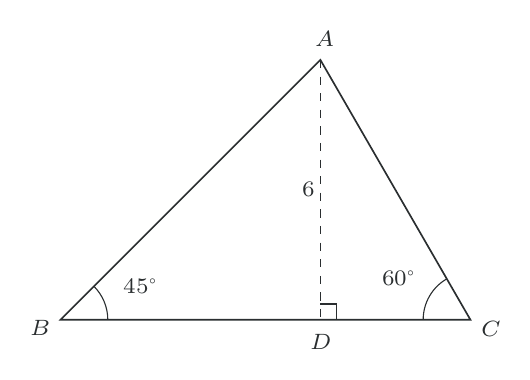
\begin{tikzpicture}[line width=0.6pt,ink,every node/.style={font=\footnotesize,inner sep=1pt}]
\draw[] (0.000mm,33.000mm) -- (-33.000mm,0.000mm) -- (19.053mm,0.000mm) -- cycle;
\draw[dashed] (0.000mm,33.000mm) -- (0.000mm,0.000mm);
\draw[line width=0.4pt] (0.000mm,2.000mm) -- (2.000mm,2.000mm) -- (2.000mm,0.000mm);
\draw[line width=0.4pt] (-27.000mm,0.000mm) arc[start angle=0.000,end angle=45.000,radius=6.000mm];
\node at (-22.837mm,4.210mm) {$45^\circ$};
\draw[line width=0.4pt] (16.053mm,5.196mm) arc[start angle=120.000,end angle=180.000,radius=6.000mm];
\node at (9.959mm,5.250mm) {$60^\circ$};
\node at (0.579mm,35.739mm) {$A$};
\node at (-35.610mm,-1.013mm) {$B$};
\node at (21.592mm,-1.179mm) {$C$};
\node at (0.000mm,-2.800mm) {$D$};
\node[left=0.5pt] at (0.000mm,16.500mm) {$6$};
\end{tikzpicture}}}{$6+6\sqrt3$}{$6+3\sqrt3$}{$6\sqrt3$}{$6+2\sqrt3$}}
\meas{S2.5}{\satg{5}{A right triangle has an acute angle $\theta$ with $\tan\theta=\dfrac{24}7$. The hypotenuse of the triangle is $50$. What is the area of the triangle?}}
\meas{S2.6}{\satq{6}{An equilateral triangle has height $15$. What is its area?}{$\dfrac{225\sqrt3}{4}$}{$75\sqrt3$}{$225$}{$150\sqrt3$}}
\meas{S2.7}{\satq{7}{In right triangle $XYZ$, the right angle is at $Y$ and $\cos Z=\dfrac7{25}$. What is the value of $\tan X$?}{$\dfrac{24}7$}{$\dfrac{25}{24}$}{$\dfrac7{24}$}{$\dfrac7{25}$}}
\meas{S2.8}{\satq{8}{A rectangle has a diagonal of length $39$. The diagonal makes an angle $\theta$ with a shorter side, where $\tan\theta=\dfrac{12}5$. What is the area of the rectangle?}{$540$}{$468$}{$270$}{$195$}}
\meas{S2.9}{\satq{9}{The altitude to the hypotenuse of an isosceles right triangle is $8\sqrt2$. What is the area of the triangle?}{$64$}{$128$}{$128\sqrt2$}{$256$}}
\meas{S2.10}{\satq{10}{In the figure, triangle $ABC$ has a right angle at $B$, and $\overline{BD}\perp\overline{AC}$. If $\sin\angle C=\dfrac5{13}$, what is $\cos\angle ABD$?\figbox{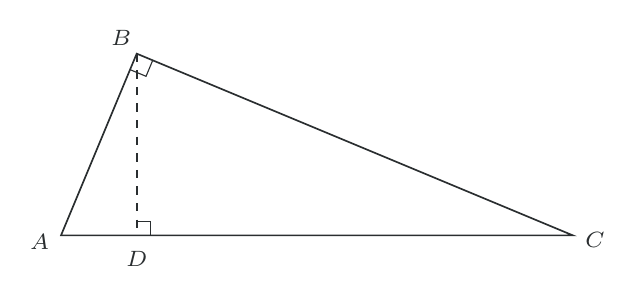
\begin{tikzpicture}[line width=0.6pt,ink,every node/.style={font=\footnotesize,inner sep=1pt}]
\draw[] (0.000mm,0.000mm) -- (9.615mm,23.077mm) -- (65.000mm,0.000mm) -- cycle;
\draw[dashed] (9.615mm,23.077mm) -- (9.615mm,0.000mm);
\draw[line width=0.4pt] (8.769mm,21.046mm) -- (10.800mm,20.200mm) -- (11.646mm,22.231mm);
\draw[line width=0.4pt] (9.615mm,1.800mm) -- (11.415mm,1.800mm) -- (11.415mm,0.000mm);
\node at (-2.675mm,-0.827mm) {$A$};
\node at (7.644mm,25.065mm) {$B$};
\node at (67.750mm,-0.527mm) {$C$};
\node at (9.615mm,-3.000mm) {$D$};
\end{tikzpicture}}}{$\dfrac{12}5$}{$\dfrac{13}{12}$}{$\dfrac{12}{13}$}{$\dfrac5{13}$}}
\meas{S2.11}{\satg{11}{In right triangle $ABC$, the right angle is at $C$, $\tan A=\dfrac34$, $BC=x+3$ and $AC=2x-2$. What is the length of $\overline{AB}$?}}
\meas{S2.12}{\satq{12}{The side lengths of a right triangle are $x$, $x+7$ and $x+8$. What is the perimeter of the triangle?}{$13$}{$17$}{$26$}{$30$}}
\meas{S2.13}{\satg{13}{In right triangle $ABC$, the right angle is at $C$ and $2\sin A=3\cos A$. The area of the triangle is $48$. What is the length of $\overline{BC}$?}}
\meas{S2.14}{\satq{14}{The perimeter of a $30^\circ$-$60^\circ$-$90^\circ$ triangle is $36+12\sqrt3$. What is the area of the triangle?}{$72\sqrt3$}{$36\sqrt3$}{$144$}{$144\sqrt3$}}
\meas{S3.1}{\satq{1}{In the figure, point $D$ lies on $\overline{AB}$ and point $E$ lies on $\overline{AC}$, with $\overline{DE}\parallel\overline{BC}$. If $AD=9$, $DB=6$ and $DE=12$, what is the length of $\overline{BC}$?\figbox{\begin{tikzpicture}[line width=0.6pt,ink,every node/.style={font=\footnotesize,inner sep=1pt}]
\draw[] (30.240mm,44.739mm) -- (0.000mm,0.000mm) -- (72.000mm,0.000mm) -- cycle;
\draw[] (12.096mm,17.895mm) -- (55.296mm,17.895mm);
\fill (12.096mm,17.895mm) circle (0.55mm);
\fill (55.296mm,17.895mm) circle (0.55mm);
\node at (29.882mm,47.516mm) {$A$};
\node at (-2.565mm,-1.122mm) {$B$};
\node at (74.606mm,-1.025mm) {$C$};
\node[left=1pt] at (12.096mm,17.895mm) {$D$};
\node[right=1pt] at (55.296mm,17.895mm) {$E$};
\node at (19.180mm,32.661mm) {$9$};
\node at (4.060mm,10.292mm) {$6$};
\node[below=0.5pt] at (33.696mm,17.895mm) {$12$};
\end{tikzpicture}}}{$8$}{$18$}{$20$}{$30$}}
\meas{S3.2}{\satq{2}{In the figure, lines $m$ and $n$ are parallel and are cut by transversal $t$. What is the value of $x$?\figbox{\begin{tikzpicture}[line width=0.6pt,ink,every node/.style={font=\footnotesize,inner sep=1pt}]
\draw[] (-25.000mm,0.000mm) -- (37.000mm,0.000mm);
\draw[] (-9.378mm,-26.000mm) -- (52.622mm,-26.000mm);
\draw[] (-4.635mm,7.715mm) -- (20.258mm,-33.715mm);
\node[right] at (37.000mm,0.000mm) {$m$};
\node[right] at (52.622mm,-26.000mm) {$n$};
\node[above left] at (-4.635mm,7.715mm) {$t$};
\draw[line width=0.4pt] (3.605mm,-6.000mm) arc[start angle=-59.000,end angle=0.000,radius=7.000mm];
\node at (17.000mm,-6.400mm) {$(3x+5)^\circ$};
\draw[line width=0.4pt] (22.622mm,-26.000mm) arc[start angle=0.000,end angle=121.000,radius=7.000mm];
\node at (32.622mm,-15.500mm) {$(7x-5)^\circ$};
\draw[line width=0.4pt] (-22.200mm,1.100mm) -- (-21.000mm,0.000mm) -- (-22.200mm,-1.100mm);
\draw[line width=0.4pt] (-6.578mm,-24.900mm) -- (-5.378mm,-26.000mm) -- (-6.578mm,-27.100mm);
\end{tikzpicture}}}{$36$}{$18$}{$9$}{$2.5$}}
\meas{S3.3}{\satg{3}{In the figure, $\angle ABC$ is a right angle, $\overline{BD}\perp\overline{AC}$, $AD=4$ and $DC=9$. What is the area of triangle $ABC$?\figbox{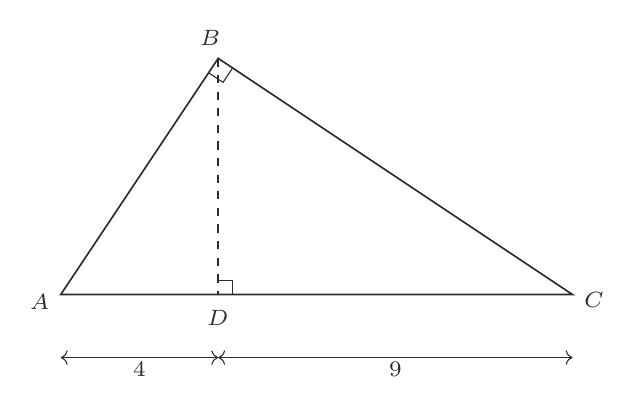
\begin{tikzpicture}[line width=0.6pt,ink,every node/.style={font=\footnotesize,inner sep=1pt}]
\draw[] (0.000mm,0.000mm) -- (20.000mm,30.000mm) -- (65.000mm,0.000mm) -- cycle;
\draw[dashed] (20.000mm,30.000mm) -- (20.000mm,0.000mm);
\draw[line width=0.4pt] (18.780mm,28.169mm) -- (20.610mm,26.949mm) -- (21.831mm,28.780mm);
\draw[line width=0.4pt] (20.000mm,1.800mm) -- (21.800mm,1.800mm) -- (21.800mm,0.000mm);
\node at (-2.640mm,-0.932mm) {$A$};
\node at (18.923mm,32.585mm) {$B$};
\node at (67.701mm,-0.737mm) {$C$};
\node at (20.000mm,-3.000mm) {$D$};
\draw[<->,line width=0.4pt] (0.000mm,-8.000mm) -- (20.000mm,-8.000mm);
\draw[<->,line width=0.4pt] (20.000mm,-8.000mm) -- (65.000mm,-8.000mm);
\node[below=0.3pt] at (10.000mm,-8.000mm) {$4$};
\node[below=0.3pt] at (42.500mm,-8.000mm) {$9$};
\end{tikzpicture}}}}
\meas{S3.4}{\satq{4}{In triangle $ABC$, points $M$ and $N$ are the midpoints of $\overline{AB}$ and $\overline{AC}$. If $MN=2x+3$ and $BC=5x-3$, what is the length of $\overline{BC}$?}{$7$}{$9$}{$21$}{$42$}}
\meas{S3.5}{\satg{5}{In the figure, $AB=AC$. The measure of $\angle A$ is $(3x-6)^\circ$ and the measure of exterior angle $\angle ACD$ is $(7x+10)^\circ$. What is the value of $x$?\figbox{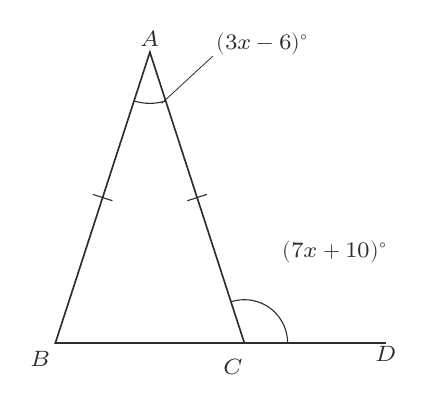
\begin{tikzpicture}[line width=0.6pt,ink,every node/.style={font=\footnotesize,inner sep=1pt}]
\draw[] (12.000mm,36.932mm) -- (0.000mm,0.000mm) -- (24.000mm,0.000mm) -- cycle;
\draw[] (24.000mm,0.000mm) -- (42.000mm,0.000mm);
\draw[line width=0.4pt] (7.236mm,18.064mm) -- (4.764mm,18.868mm);
\draw[line width=0.4pt] (19.236mm,18.868mm) -- (16.764mm,18.064mm);
\node at (-1.954mm,-2.005mm) {$B$};
\node at (22.500mm,-3.000mm) {$C$};
\node[below] at (42.000mm,0.000mm) {$D$};
\node[above=0.3mm] at (12.000mm,36.932mm) {$A$};
\draw[line width=0.4pt] (9.991mm,30.750mm) arc[start angle=-108.000,end angle=-72.000,radius=6.500mm];
\draw[line width=0.3pt] (20.000mm,36.432mm) -- (13.500mm,30.432mm);
\node[right=0pt] at (20.000mm,37.932mm) {$(3x-6)^\circ$};
\draw[line width=0.4pt] (29.500mm,0.000mm) arc[start angle=0.000,end angle=108.000,radius=5.500mm];
\node at (35.500mm,11.500mm) {$(7x+10)^\circ$};
\end{tikzpicture}}}}
\meas{S3.6}{\satg{6}{The side lengths of a triangle are $9$, $14$ and $3x$, where $x$ is a positive integer. How many possible values of $x$ are there?}}
\meas{S3.7}{\satq{7}{In the figure, convex pentagon $ABCDE$ has $\overline{AB}\parallel\overline{ED}$. The angles are $\angle B=(2x+45)^\circ$, $\angle C=(3x+20)^\circ$ and $\angle D=(x+55)^\circ$. What is the measure of $\angle C$?\figbox{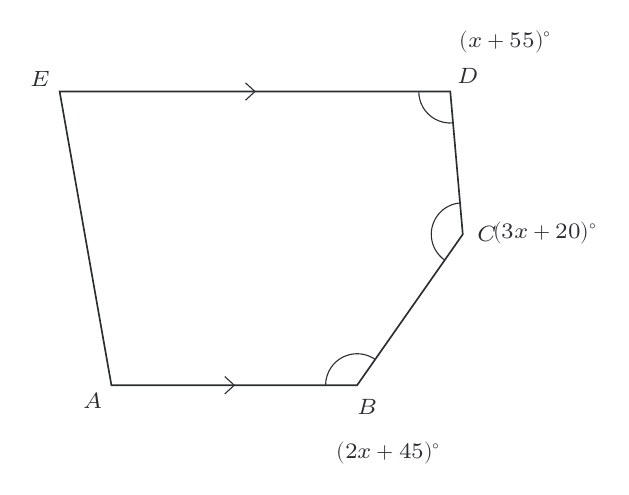
\begin{tikzpicture}[line width=0.6pt,ink,every node/.style={font=\footnotesize,inner sep=1pt}]
\draw[] (0.000mm,0.000mm) -- (31.200mm,0.000mm) -- (44.622mm,19.168mm) -- (43.035mm,37.299mm) -- (-6.577mm,37.299mm) -- cycle;
\draw[line width=0.4pt] (14.400mm,1.100mm) -- (15.600mm,0.000mm) -- (14.400mm,-1.100mm);
\draw[line width=0.4pt] (17.029mm,38.399mm) -- (18.229mm,37.299mm) -- (17.029mm,36.199mm);
\node at (-2.303mm,-1.923mm) {$A$};
\node at (32.468mm,-2.719mm) {$B$};
\node at (47.621mm,19.224mm) {$C$};
\node at (45.264mm,39.307mm) {$D$};
\node at (-9.105mm,38.914mm) {$E$};
\draw[line width=0.4pt] (33.494mm,3.277mm) arc[start angle=55.000,end angle=180.000,radius=4.000mm];
\node at (35.215mm,-8.610mm) {$(2x+45)^\circ$};
\draw[line width=0.4pt] (44.273mm,23.153mm) arc[start angle=-265.000,end angle=-125.000,radius=4.000mm];
\node at (55.120mm,19.365mm) {$(3x+20)^\circ$};
\draw[line width=0.4pt] (39.035mm,37.299mm) arc[start angle=-180.000,end angle=-85.000,radius=4.000mm];
\node at (50.093mm,43.659mm) {$(x+55)^\circ$};
\end{tikzpicture}}}{$140^\circ$}{$125^\circ$}{$95^\circ$}{$40^\circ$}}
\meas{S3.8}{\satq{8}{In triangle $ABC$, point $D$ is on $\overline{AB}$ and point $E$ is on $\overline{AC}$ with $\overline{DE}\parallel\overline{BC}$ and $AD:DB=2:3$. The area of triangle $ABC$ is $100$. What is the area of quadrilateral $DBCE$?}{$16$}{$40$}{$60$}{$84$}}
\meas{S3.9}{\satq{9}{In triangle $ABC$, medians $\overline{AD}$ and $\overline{BE}$ meet at $G$. If $AG=4x+2$ and $GD=x+7$, what is the length of $\overline{AD}$?}{$13$}{$26$}{$39$}{$52$}}
\meas{S3.10}{\satqw{10}{A triangle has side lengths $9$, $12$ and $14$. Which statement about its largest angle is true?}{It is less than $90^\circ$.}{It measures exactly $90^\circ$.}{It is greater than $90^\circ$.}{Its measure cannot be found from the side lengths.}}
\meas{S3.11}{\satq{11}{In the figure, segments $\overline{AD}$ and $\overline{BC}$ intersect at $E$, and $\overline{AB}\parallel\overline{DC}$. If $AE=12$, $ED=18$ and $BE=10$, what is the length of $\overline{BC}$?\figbox{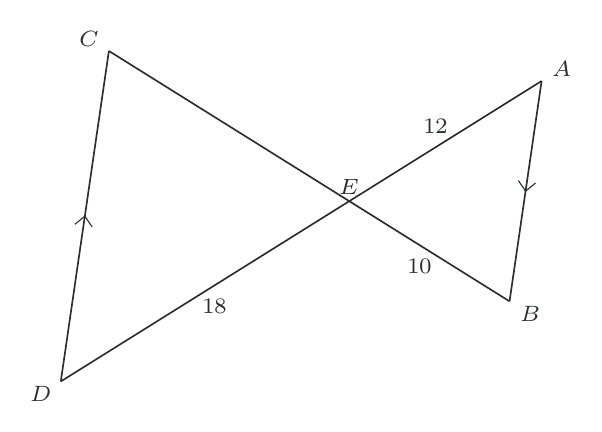
\begin{tikzpicture}[line width=0.6pt,ink,every node/.style={font=\footnotesize,inner sep=1pt}]
\draw[] (24.424mm,15.262mm) -- (-36.636mm,-22.893mm);
\draw[] (20.353mm,-12.718mm) -- (-30.530mm,19.077mm);
\draw[] (24.424mm,15.262mm) -- (20.353mm,-12.718mm);
\draw[] (-36.636mm,-22.893mm) -- (-30.530mm,19.077mm);
\draw[line width=0.4pt] (23.650mm,2.301mm) -- (22.388mm,1.272mm) -- (21.473mm,2.618mm);
\draw[line width=0.4pt] (-34.844mm,-2.937mm) -- (-33.583mm,-1.908mm) -- (-32.667mm,-3.254mm);
\node at (26.968mm,16.851mm) {$A$};
\node at (22.897mm,-14.308mm) {$B$};
\node at (-33.074mm,20.667mm) {$C$};
\node at (-39.180mm,-24.482mm) {$D$};
\node[above=1pt] at (0.000mm,0.000mm) {$E$};
\node at (10.993mm,9.581mm) {$12$};
\node at (-17.099mm,-13.397mm) {$18$};
\node at (8.958mm,-8.310mm) {$10$};
\end{tikzpicture}}}{$15$}{$\dfrac{50}{3}$}{$22$}{$25$}}
\meas{S3.12}{\satq{12}{Each interior angle of a regular polygon measures $(4x+10)^\circ$ and each exterior angle measures $(x-5)^\circ$. How many sides does the polygon have?}{$6$}{$12$}{$30$}{$35$}}
\meas{S3.13}{\satg{13}{Two similar triangles have perimeters $24$ and $40$. The larger triangle has area $250$. What is the area of the smaller triangle?}}
\meas{S3.14}{\satq{14}{In the figure, triangle $ABC$ has $AB=AC$, and point $D$ lies on $\overline{AC}$ so that $AD=BD=BC$. What is the measure of $\angle ABC$?\figbox{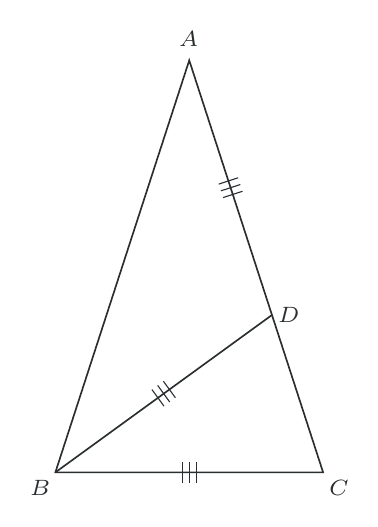
\begin{tikzpicture}[line width=0.6pt,ink,every node/.style={font=\footnotesize,inner sep=1pt}]
\draw[] (17.000mm,52.321mm) -- (0.000mm,0.000mm) -- (34.000mm,0.000mm) -- cycle;
\draw[] (0.000mm,0.000mm) -- (27.507mm,19.985mm);
\draw[line width=0.4pt] (23.212mm,37.410mm) -- (20.739mm,36.607mm);
\draw[line width=0.4pt] (23.490mm,36.554mm) -- (21.017mm,35.751mm);
\draw[line width=0.4pt] (23.768mm,35.698mm) -- (21.295mm,34.895mm);
\draw[line width=0.4pt] (12.261mm,10.515mm) -- (13.789mm,8.412mm);
\draw[line width=0.4pt] (12.989mm,11.044mm) -- (14.517mm,8.941mm);
\draw[line width=0.4pt] (13.717mm,11.573mm) -- (15.246mm,9.470mm);
\draw[line width=0.4pt] (16.100mm,1.300mm) -- (16.100mm,-1.300mm);
\draw[line width=0.4pt] (17.000mm,1.300mm) -- (17.000mm,-1.300mm);
\draw[line width=0.4pt] (17.900mm,1.300mm) -- (17.900mm,-1.300mm);
\node at (17.000mm,55.121mm) {$A$};
\node at (-1.954mm,-2.005mm) {$B$};
\node at (35.954mm,-2.005mm) {$C$};
\node[right=1pt] at (27.507mm,19.985mm) {$D$};
\end{tikzpicture}}}{$36^\circ$}{$60^\circ$}{$72^\circ$}{$108^\circ$}}
\meas{S4.1}{\satq{1}{In the figure, $AB=13$, $BC=20$ and $AC=21$. What is the area of triangle $ABC$?\figbox{\begin{tikzpicture}[line width=0.6pt,ink,every node/.style={font=\footnotesize,inner sep=1pt}]
\draw[] (0.000mm,0.000mm) -- (17.000mm,40.800mm) -- (71.400mm,0.000mm) -- cycle;
\node at (-2.542mm,-1.173mm) {$A$};
\node at (15.833mm,43.345mm) {$B$};
\node at (74.063mm,-0.864mm) {$C$};
\node at (6.100mm,21.400mm) {$13$};
\node at (45.760mm,22.480mm) {$20$};
\node at (35.700mm,-2.600mm) {$21$};
\end{tikzpicture}}}{$126$}{$130$}{$136.5$}{$210$}}
\meas{S4.2}{\satq{2}{A tower stands on level ground. Points $A$ and $B$ are on the ground in line with the base $O$ of the tower, with $A$ between $B$ and $O$ and $AB=40$ meters. The angle of elevation of the top $T$ of the tower is $45^\circ$ from $A$ and $30^\circ$ from $B$. What is the height of the tower, in meters?\figbox{\begin{tikzpicture}[line width=0.6pt,ink,every node/.style={font=\footnotesize,inner sep=1pt}]
\draw[] (-77.820mm,0.000mm) -- (7.000mm,0.000mm);
\draw[] (0.000mm,0.000mm) -- (0.000mm,42.620mm);
\draw[] (-73.820mm,0.000mm) -- (0.000mm,42.620mm);
\draw[] (-42.620mm,0.000mm) -- (0.000mm,42.620mm);
\draw[line width=0.4pt] (0.000mm,2.200mm) -- (-2.200mm,2.200mm) -- (-2.200mm,0.000mm);
\node[above] at (0.000mm,42.620mm) {$T$};
\node[below] at (-73.820mm,0.000mm) {$B$};
\node[below] at (-42.620mm,0.000mm) {$A$};
\node[below] at (0.000mm,0.000mm) {$O$};
\fill (-42.620mm,0.000mm) circle (0.55mm);
\fill (-73.820mm,0.000mm) circle (0.55mm);
\draw[line width=0.4pt] (-64.820mm,0.000mm) arc[start angle=0.000,end angle=30.000,radius=9.000mm];
\node at (-57.820mm,2.000mm) {$30^\circ$};
\draw[line width=0.4pt] (-36.620mm,0.000mm) arc[start angle=0.000,end angle=45.000,radius=6.000mm];
\node at (-31.620mm,4.000mm) {$45^\circ$};
\draw[<->,line width=0.4pt] (-73.820mm,-7.300mm) -- (-42.620mm,-7.300mm);
\node[below] at (-58.220mm,-7.000mm) {$40$ m};
\end{tikzpicture}}}{$40\sqrt3$}{$20(\sqrt3+1)$}{$20\sqrt3$}{$40(\sqrt3-1)$}}
\meas{S4.3}{\satq{3}{A $25$-foot ladder leans against a vertical wall with its top $24$ feet above the ground. The foot of the ladder is pulled away from the wall until the top of the ladder is $20$ feet above the ground. How many feet did the foot of the ladder move?}{$22$}{$15$}{$8$}{$4$}}
\meas{S4.4}{\satg{4}{In the $xy$-plane, $P=(-2,1)$ and $R=(7,-2)$. Point $Q$ has coordinates $(4,k)$, and $\angle PQR$ is a right angle. What is the sum of all possible values of $k$?\figbox{\begin{tikzpicture}[line width=0.6pt,ink,every node/.style={font=\footnotesize,inner sep=1pt}]
\draw[->,line width=0.4pt] (-15.840mm,0.000mm) -- (38.720mm,0.000mm);
\draw[->,line width=0.4pt] (0.000mm,-29.040mm) -- (0.000mm,20.240mm);
\node[right] at (38.720mm,0.000mm) {$x$};
\node[above] at (0.000mm,20.240mm) {$y$};
\draw[line width=0.3pt] (-13.200mm,-0.900mm) -- (-13.200mm,0.900mm);
\draw[line width=0.3pt] (-8.800mm,-0.900mm) -- (-8.800mm,0.900mm);
\draw[line width=0.3pt] (-4.400mm,-0.900mm) -- (-4.400mm,0.900mm);
\draw[line width=0.3pt] (4.400mm,-0.900mm) -- (4.400mm,0.900mm);
\draw[line width=0.3pt] (8.800mm,-0.900mm) -- (8.800mm,0.900mm);
\draw[line width=0.3pt] (13.200mm,-0.900mm) -- (13.200mm,0.900mm);
\draw[line width=0.3pt] (17.600mm,-0.900mm) -- (17.600mm,0.900mm);
\draw[line width=0.3pt] (22.000mm,-0.900mm) -- (22.000mm,0.900mm);
\draw[line width=0.3pt] (26.400mm,-0.900mm) -- (26.400mm,0.900mm);
\draw[line width=0.3pt] (30.800mm,-0.900mm) -- (30.800mm,0.900mm);
\draw[line width=0.3pt] (35.200mm,-0.900mm) -- (35.200mm,0.900mm);
\draw[line width=0.3pt] (-0.900mm,-26.400mm) -- (0.900mm,-26.400mm);
\draw[line width=0.3pt] (-0.900mm,-22.000mm) -- (0.900mm,-22.000mm);
\draw[line width=0.3pt] (-0.900mm,-17.600mm) -- (0.900mm,-17.600mm);
\draw[line width=0.3pt] (-0.900mm,-13.200mm) -- (0.900mm,-13.200mm);
\draw[line width=0.3pt] (-0.900mm,-8.800mm) -- (0.900mm,-8.800mm);
\draw[line width=0.3pt] (-0.900mm,-4.400mm) -- (0.900mm,-4.400mm);
\draw[line width=0.3pt] (-0.900mm,4.400mm) -- (0.900mm,4.400mm);
\draw[line width=0.3pt] (-0.900mm,8.800mm) -- (0.900mm,8.800mm);
\draw[line width=0.3pt] (-0.900mm,13.200mm) -- (0.900mm,13.200mm);
\draw[line width=0.3pt] (-0.900mm,17.600mm) -- (0.900mm,17.600mm);
\draw[dashed] (17.600mm,-27.280mm) -- (17.600mm,18.480mm);
\node[above right] at (17.600mm,13.200mm) {$x=4$};
\draw[] (-8.800mm,4.400mm) -- (30.800mm,-8.800mm);
\fill (-8.800mm,4.400mm) circle (0.55mm);
\node[above left] at (-8.800mm,4.400mm) {$P({-}2,1)$};
\fill (30.800mm,-8.800mm) circle (0.55mm);
\node[below right] at (30.800mm,-8.800mm) {$R(7,{-}2)$};
\end{tikzpicture}}}}
\meas{S4.5}{\satg{5}{In the $xy$-plane, $A=(1,1)$, $B=(13,1)$ and $C=(7,k)$, where $k>0$. The area of triangle $ABC$ is $48$. What is the perimeter of triangle $ABC$?}}
\meas{S4.6}{\satq{6}{The figure is a rectangle topped by an isosceles triangle. The rectangle measures $12$ by $6$, and each of the two equal sides of the triangle is $10$. What is the area of the whole figure?\figbox{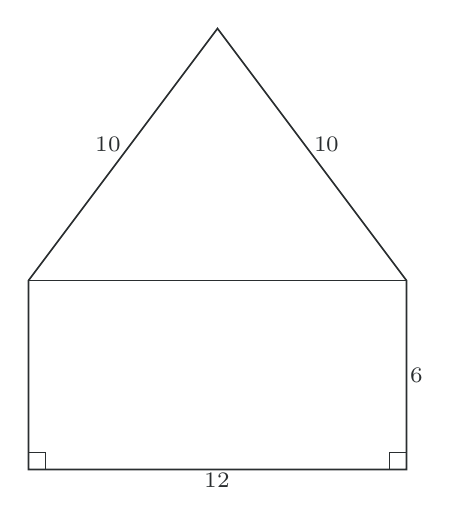
\begin{tikzpicture}[line width=0.6pt,ink,every node/.style={font=\footnotesize,inner sep=1pt}]
\draw[] (0.000mm,0.000mm) -- (48.000mm,0.000mm) -- (48.000mm,24.000mm) -- (24.000mm,56.000mm) -- (0.000mm,24.000mm) -- cycle;
\draw[] (0.000mm,24.000mm) -- (48.000mm,24.000mm);
\draw[line width=0.4pt] (2.200mm,0.000mm) -- (2.200mm,2.200mm) -- (0.000mm,2.200mm);
\draw[line width=0.4pt] (48.000mm,2.200mm) -- (45.800mm,2.200mm) -- (45.800mm,0.000mm);
\node[below] at (24.000mm,0.000mm) {$12$};
\node[right] at (48.000mm,12.000mm) {$6$};
\node[above left=-0.5pt] at (12.000mm,40.000mm) {$10$};
\node[above right=-0.5pt] at (36.000mm,40.000mm) {$10$};
\end{tikzpicture}}}{$48$}{$120$}{$132$}{$168$}}
\meas{S4.7}{\satq{7}{A vertical pole stands on level ground. Two straight cables run from the top of the pole to points $A$ and $B$ on the ground on opposite sides of the pole. The cables are $17$ meters and $10$ meters long, and $A$ and $B$ are $21$ meters apart. How tall is the pole, in meters?}{$6$}{$9$}{$15$}{$8$}}
\meas{S4.8}{\satg{8}{In the figure, $\angle ABC$ and $\angle ACD$ are right angles, $AB=9$, $\tan\angle BAC=\dfrac43$ and $\sin\angle CAD=\dfrac45$. What is the perimeter of quadrilateral $ABCD$?\figbox{\begin{tikzpicture}[line width=0.6pt,ink,every node/.style={font=\footnotesize,inner sep=1pt}]
\draw[] (0.000mm,27.000mm) -- (0.000mm,0.000mm) -- (36.000mm,0.000mm) -- (72.000mm,48.000mm) -- cycle;
\draw[] (0.000mm,27.000mm) -- (36.000mm,0.000mm);
\draw[line width=0.4pt] (0.000mm,2.200mm) -- (2.200mm,2.200mm) -- (2.200mm,0.000mm);
\draw[line width=0.4pt] (34.240mm,1.320mm) -- (35.560mm,3.080mm) -- (37.320mm,1.760mm);
\node at (-2.869mm,27.877mm) {$A$};
\node at (-2.464mm,-1.711mm) {$B$};
\node at (37.298mm,-2.705mm) {$C$};
\node at (74.515mm,49.635mm) {$D$};
\node[left] at (0.000mm,13.500mm) {$9$};
\end{tikzpicture}}}}
\meas{S4.9}{\satq{9}{A lamp is fixed to the top of a vertical post on level ground. A person $1.5$ m tall stands $6$ m from the post and casts a shadow $2$ m long (the shadow points away from the post). The person then walks directly away from the post until the shadow is $4$ m long. How many meters did the person walk?}{$2$}{$4$}{$6$}{$12$}}
\meas{S4.10}{\satq{10}{Point $A=(2,-1)$ and point $B=(8,7)$. Which of the following points lies on the perpendicular bisector of $\overline{AB}$?}{$(9,0)$}{$(9,6)$}{$(8,-1)$}{$(6,-4)$}}
\meas{S4.11}{\satq{11}{A rectangle has a diagonal of length $25$, and its two side lengths differ by $5$. What is the perimeter of the rectangle?}{$100$}{$70$}{$50$}{$35$}}
\meas{S4.12}{\satq{12}{An isosceles triangle has a base of $16$ and a perimeter of $36$. What is its area?}{$96$}{$80$}{$64$}{$48$}}
\meas{S4.13}{\satg{13}{In the figure, a square is placed inside right triangle $ABC$ with one vertex at the right-angle vertex $C$ and the opposite vertex on the hypotenuse $\overline{AB}$. The legs are $CB=12$ and $CA=6$. What is the side length of the square?\figbox{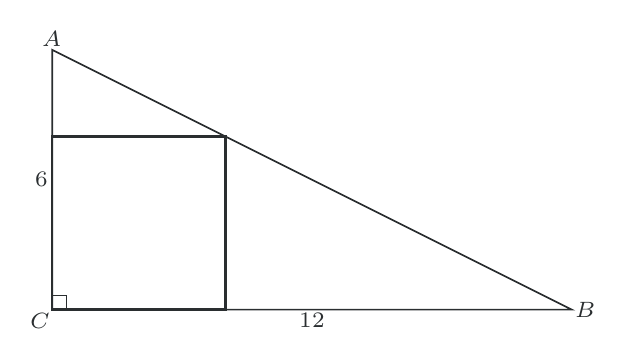
\begin{tikzpicture}[line width=0.6pt,ink,every node/.style={font=\footnotesize,inner sep=1pt}]
\draw[] (0.000mm,0.000mm) -- (66.000mm,0.000mm) -- (0.000mm,33.000mm) -- cycle;
\draw[line width=0.9pt] (0.000mm,0.000mm) -- (22.000mm,0.000mm) -- (22.000mm,22.000mm) -- (0.000mm,22.000mm) -- cycle;
\draw[line width=0.4pt] (1.800mm,0.000mm) -- (1.800mm,1.800mm) -- (0.000mm,1.800mm);
\node[below] at (33.000mm,0.000mm) {$12$};
\node[left] at (0.000mm,16.500mm) {$6$};
\node[below left] at (0.000mm,0.000mm) {$C$};
\node[right] at (66.000mm,0.000mm) {$B$};
\node[above] at (0.000mm,33.000mm) {$A$};
\end{tikzpicture}}}}
\meas{S4.14}{\satq{14}{A rectangular box measures $6$ by $8$ by $24$. What is the length of the longest segment that can be drawn between two corners of the box?}{$676$}{$38$}{$26$}{$10$}}
\meas{S5.1}{\satq{1}{In right triangle $ABC$, the right angle is at $C$, and $\overline{CH}$ is the altitude to hypotenuse $\overline{AB}$ with $H$ on $\overline{AB}$. If $CH=12$, $AH=x$ and $HB=x+7$, what is the perimeter of triangle $ABC$?}{$25$}{$37$}{$49$}{$60$}}
\meas{S5.2}{\satg{2}{In right triangle $ABC$, the right angle is at $C$. The area of the triangle is $6$, and $\tan A+\tan B=\dfrac{25}{12}$. What is the length of the hypotenuse?}}
\meas{S5.3}{\satq{3}{In trapezoid $ABCD$, $\overline{AB}\parallel\overline{CD}$, $AB=8$ and $CD=12$. The diagonals meet at $E$, and the area of triangle $CDE$ is $90$. What is the area of triangle $ABE$?}{$40$}{$50$}{$60$}{$135$}}
\meas{S5.4}{\satg{4}{Two sides of a triangle measure $7$ and $8$, and the third side has integer length $x$. For how many values of $x$ is the triangle obtuse?}}
\meas{S5.5}{\satq{5}{A circle is inscribed in a right triangle with legs $9$ and $12$, touching all three sides. What is the area of the circle?}{$\dfrac{9\pi}{4}$}{$9\pi$}{$36\pi$}{$\dfrac{225\pi}{4}$}}
\meas{S5.6}{\satq{6}{In the $xy$-plane, point $P$ lies on the line $y=\dfrac34x$ in the first quadrant, and $P$ is $20$ units from the origin. What is the sum of the coordinates of $P$?}{$7$}{$20$}{$28$}{$35$}}
\meas{S5.7}{\satq{7}{Two vertical poles of heights $12$ m and $20$ m stand $15$ m apart on level ground. A cable runs from the top of each pole to the base of the other, and the cables cross at point $X$. How many meters above the ground is $X$?\figbox{\begin{tikzpicture}[line width=0.6pt,ink,every node/.style={font=\footnotesize,inner sep=1pt}]
\draw[] (-5.000mm,0.000mm) -- (50.000mm,0.000mm);
\draw[] (0.000mm,0.000mm) -- (0.000mm,36.000mm);
\draw[] (45.000mm,0.000mm) -- (45.000mm,60.000mm);
\draw[line width=0.5pt] (0.000mm,0.000mm) -- (45.000mm,60.000mm);
\draw[line width=0.5pt] (45.000mm,0.000mm) -- (0.000mm,36.000mm);
\node[left] at (0.000mm,18.000mm) {$12$};
\node[right] at (45.000mm,30.000mm) {$20$};
\node[below] at (22.500mm,0.000mm) {$15$};
\fill (0.000mm,36.000mm) circle (0.55mm);
\fill (45.000mm,60.000mm) circle (0.55mm);
\end{tikzpicture}}}{$7.5$}{$16$}{$32$}{$240$}}
\meas{S5.8}{\satg{8}{The side lengths of a right triangle form an arithmetic sequence, and the area of the triangle is $54$. What is the perimeter of the triangle?}}
\meas{S5.9}{\satq{9}{A regular hexagon $ABCDEF$ has side length $6$. Triangle $ACE$ is formed by joining alternate vertices. What is the area of triangle $ACE$?\figbox{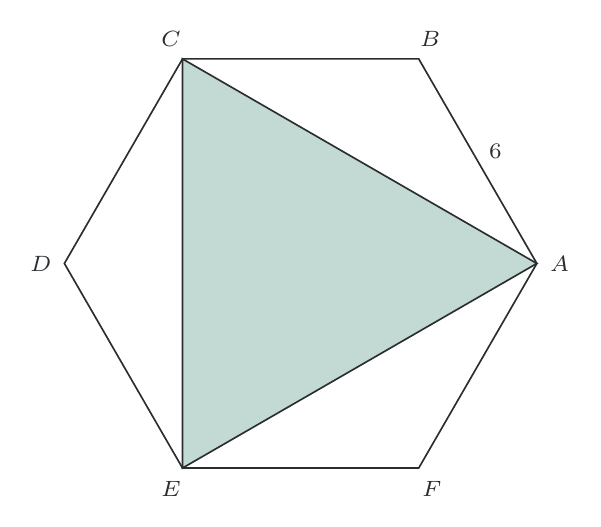
\begin{tikzpicture}[line width=0.6pt,ink,every node/.style={font=\footnotesize,inner sep=1pt}]
\fill[accent!25] (30.000mm,0.000mm) -- (-15.000mm,25.981mm) -- (-15.000mm,-25.981mm) -- cycle;
\draw[] (30.000mm,0.000mm) -- (15.000mm,25.981mm) -- (-15.000mm,25.981mm) -- (-30.000mm,0.000mm) -- (-15.000mm,-25.981mm) -- (15.000mm,-25.981mm) -- cycle;
\draw[] (30.000mm,0.000mm) -- (-15.000mm,25.981mm) -- (-15.000mm,-25.981mm) -- cycle;
\node at (33.000mm,0.000mm) {$A$};
\node at (16.500mm,28.579mm) {$B$};
\node at (-16.500mm,28.579mm) {$C$};
\node at (-33.000mm,0.000mm) {$D$};
\node at (-16.500mm,-28.579mm) {$E$};
\node at (16.500mm,-28.579mm) {$F$};
\node at (24.752mm,14.290mm) {$6$};
\end{tikzpicture}}}{$54\sqrt3$}{$27\sqrt3$}{$18\sqrt3$}{$9\sqrt3$}}
\meas{S5.10}{\satq{10}{In a regular decagon (a polygon with $10$ equal sides and equal angles) $ABCDEFGHIJ$, what is the measure of $\angle ACD$?}{$162^\circ$}{$144^\circ$}{$126^\circ$}{$18^\circ$}}
\meas{S5.11}{\satg{11}{Rectangle $ABCD$ has $AB=12$ and $BC=16$. The perpendicular from $A$ to diagonal $\overline{BD}$ meets $\overline{BD}$ at $H$. What is the value of $DH-BH$?}}
\meas{S5.12}{\satq{12}{From the top of a vertical tower $30$ m tall, the angles of depression of two cars on the level road, in line with the base of the tower and on opposite sides of it, are $45^\circ$ and $30^\circ$. How far apart are the cars, in meters?}{$30\sqrt3-30$}{$30\sqrt3$}{$60$}{$30+30\sqrt3$}}
\meas{S5.13}{\satq{13}{In parallelogram $ABCD$, $AB=14$, $AD=10$ and $\angle A=60^\circ$. What is the area of the parallelogram?}{$140$}{$70\sqrt3$}{$70$}{$35\sqrt3$}}
\meas{S5.14}{\satg{14}{An isosceles triangle has two sides of length $25$ and an area of $168$. What is the sum of all possible lengths of the third side?}}
\meas{S5.15}{\satq{15}{In isosceles trapezoid $ABCD$, $\overline{AB}\parallel\overline{DC}$, $AB=10$, $DC=26$ and $AD=BC=10$. What is the area of the trapezoid?\figbox{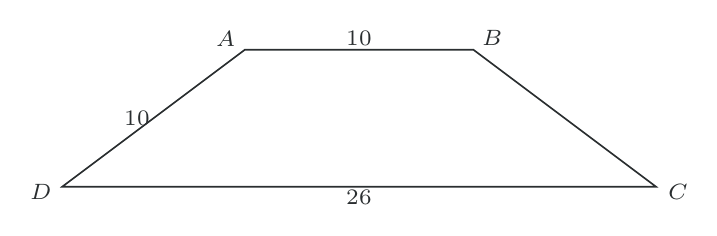
\begin{tikzpicture}[line width=0.6pt,ink,every node/.style={font=\footnotesize,inner sep=1pt}]
\draw[] (0.000mm,0.000mm) -- (75.400mm,0.000mm) -- (52.200mm,17.400mm) -- (23.200mm,17.400mm) -- cycle;
\node at (-2.728mm,-0.630mm) {$D$};
\node at (78.128mm,-0.630mm) {$C$};
\node at (54.601mm,18.841mm) {$B$};
\node at (20.799mm,18.841mm) {$A$};
\node[above] at (37.700mm,17.400mm) {$10$};
\node[below] at (37.700mm,0.000mm) {$26$};
\node[left] at (11.600mm,8.700mm) {$10$};
\end{tikzpicture}}}{$108$}{$156$}{$180$}{$216$}}
\meas{S5.16}{\satq{16}{In right triangle $ABC$, the right angle is at $B$ and the legs are $AB=9$ and $BC=12$. Point $D$ is on $\overline{AB}$ and point $E$ is on $\overline{BC}$ with $\overline{DE}\parallel\overline{AC}$, and the area of triangle $DBE$ is one-fourth the area of triangle $ABC$. What is the length of $\overline{DE}$?}{$3.75$}{$11.25$}{$30$}{$7.5$}}
\meas{S5.17}{\satq{17}{Square $ABCD$ has side length $12$. Point $E$ is the midpoint of $\overline{AB}$ and point $F$ is the midpoint of $\overline{BC}$. What is the area of triangle $DEF$?}{$54$}{$36$}{$72$}{$90$}}
\meas{S5.18}{\satq{18}{In the figure, triangle $ABC$ has a right angle at $C$ and $\tan B=\dfrac12$. Point $D$ is on $\overline{BC}$ with $BD=4$ and $DC=6$. What is $\tan\angle ADC$?\figbox{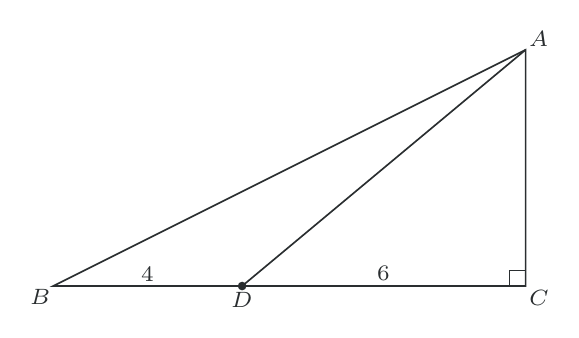
\begin{tikzpicture}[line width=0.6pt,ink,every node/.style={font=\footnotesize,inner sep=1pt}]
\draw[] (60.000mm,30.000mm) -- (0.000mm,0.000mm) -- (60.000mm,0.000mm) -- cycle;
\draw[] (60.000mm,30.000mm) -- (24.000mm,0.000mm);
\fill (24.000mm,0.000mm) circle (0.55mm);
\draw[line width=0.4pt] (60.000mm,2.000mm) -- (58.000mm,2.000mm) -- (58.000mm,0.000mm);
\node[below left] at (0.000mm,0.000mm) {$B$};
\node[below right] at (60.000mm,0.000mm) {$C$};
\node[above right] at (60.000mm,30.000mm) {$A$};
\node[below=1pt] at (24.000mm,0.000mm) {$D$};
\node[above=0.5pt] at (12.000mm,0.000mm) {$4$};
\node[above=0.5pt] at (42.000mm,0.000mm) {$6$};
\end{tikzpicture}}}{$\dfrac12$}{$\dfrac65$}{$\dfrac54$}{$\dfrac56$}}
\meas{S5.19}{\satg{19}{In the $xy$-plane, point $P$ lies on the $x$-axis and is equally distant from $A=(0,6)$ and $B=(8,2)$. What is the area of triangle $PAB$?}}
\meas{S5.20}{\satq{20}{Which of the following lists of side lengths forms a right triangle?}{$9,\ 40,\ 41$}{$8,\ 15,\ 16$}{$12,\ 35,\ 36$}{$20,\ 21,\ 28$}}
\meas{K}{\setkicker{Set 2}{Chained geometry: coordinates, composite figures, word problems.}}
\immediate\closeout\mw
\end{document}